\documentclass{beamer}[10]


%
% macro
%

\usepackage[orientation=landscape,size=custom,width=16,height=9,scale=0.5,debug]{beamerposter} 
\usepackage[beamer]{hf-tikz}
\usepackage{xfrac}
\usepackage[usenames,dvipsnames]{color}
\usepackage{makeidx}

%
% Macros
%

\definecolor{light-gray}{gray}{.80}
\definecolor{light-yellow}{rgb}{255,255,153}

% colorized font
\newcommand{\red}[1] { {\color{red} #1} }
\newcommand{\blue}[1] { {\color{blue} #1} }
\newcommand{\green}[1] { {\color{green} #1} }
\newcommand{\gray}[1] { {\color{gray} #1} }
\newcommand{\grey}[1] { {\color{gray} #1} }


% environments
\newminted{python}{mathescape} 
\newenvironment{theindex}
 {\let\item\par
  %definitions for subitem etc
  }{}
\newcommand\indexspace{}
\newenvironment{xframe}[2][]
  {\begin{frame}[fragile,environment=xframe,#1]
  \frametitle{#2}}
  {\end{frame}}
  
% python highlights: module, method
\newcommand{\pymodule}[1] { \textbf{#1} }
\newcommand{\pyfunction}[1] {\textit{#1}}
\newcommand{\keyword}[1] {\texttt{#1}}
\newcommand{\pyver}[1]{\colorbox{yellow}{#1}}
\newcommand{\pyvers}[1]{\raisebox{0em}{\colorbox{yellow}{#1}}}

% special symbils
\newcommand{\mymapsto}{\operatornamewithlimits{\longmapsto}}

\makeatletter
\newcommand{\xMapsto}[2][]{\ext@arrow 0599{\Mapstofill@}{#1}{#2}}
\def\Mapstofill@{\arrowfill@{\Mapstochar\Relbar}\Relbar\Rightarrow}
\makeatother

\newcommand{\code}[1] { \texttt{#1} }


%
% style
%

\setbeamercovered{transparent}
\mode<presentation>

%\geometry{top=5pt, margin=5pt}
%The outertheme defines the head and the footline of each slide
% \setbeamercolor{block title}{bg=orange}
% \useinnertheme{circles}
% \useoutertheme{split}
%\beamertemplatenavigationsymbolsempty

%\usetheme[numbers,totalnumber,compress,sidebarshades]{Babel}
\setbeamertemplate{headline}{
 \leavevmode%
  \hbox{%
%,bb=0 0 5cm 2cm
    \hskip5pt
    
\includegraphics[height=1.2cm]{babel-logo.eps}
    \hskip245pt
    
\includegraphics[height=1.2cm]{ep14-logo.eps}
    }
}
\setbeamertemplate{footline}{
    \centerline{
        \gray{
            Roberto Polli - \href{mailto:roberto.polli@babel.it}{roberto.polli@babel.it}
        }
    }
}
%\useinnertheme[shadow=false]{rounded}
% frametitle
\setbeamertemplate{frametitle}[default][center]
\setbeamercolor*{frametitle}{bg=white,fg=gray,parent=palette primary}
\setbeamerfont{frametitle}{series=\bfseries,size={\fontsize{16}{8}}}
%title
\setbeamercolor{title}{fg=black,bg=white}
\setbeamerfont{title}{series=\bfseries,size={\fontsize{24.88}{32}}}
%subtitle
\setbeamercolor{subtitle}{fg=gray}
\setbeamerfont{subtitle}{series=\bfseries,size={\fontsize{14}{}}}
%titlepage
\setbeamertemplate{title page}[default][center]
% bullets
\setbeamercolor{itemize item}{fg=gray}
\setbeamertemplate{itemize items}[circle]
\setbeamercolor{itemize item}{fg=light-gray}
\setbeamercolor{itemize items}{fg=light-gray}
% enumerations
\setbeamercolor{enumerate item}{fg=black}
\setbeamercolor{local structure}{fg=black}

%
% increase itemize spacing
%
%\newlength{\wideitemsep}
%\setlength{\wideitemsep}{\itemsep}
%\addtolength{\wideitemsep}{14pt}
%\let\olditem\item
%\renewcommand{\item}{\setlength{\itemsep}{\wideitemsep}\olditem}

  % \usecolortheme[named=orange]{structure}
  % \useinnertheme{circles}
  % \usefonttheme[onlymath]{serif}
  \setbeamercovered{transparent}
  % \setbeamertemplate{blocks}[rounded][shadow=true]

\makeindex


\title{Python for System Administrator}
\subtitle{EuroPython 2014, $24^{th}$ July - Berlin}
\author{Roberto Polli - \href{mailto:roberto.polli@babel.it}{roberto.polli@babel.it}}
\date{24 July 2014}
\institute{Babel Srl P.zza S. Benedetto da Norcia, 33\\ 
    00040, Pomezia (RM) - www.babel.it}

%
%
\begin{document}

%% cover
\frame{\titlepage 
\vspace{-0.5cm}
}

%% agenda
\frame{\frametitle{Agenda}
\tiny
\tableofcontents%[pausesection]
}


%\section{Test}
\usepackage{pdfcomment}

\begin{pyframe}{Title}
Antani
module: \pymodule{subprocess, psutil}
symbols: $\clubsuit \diamondsuit \heartsuit \spadesuit$
\end{pyframe}

\begin{pyframe}{\pyoptional{Test Slide with styles}}
\begin{itemize}
\item Bullet \index{Bullet} item 0 $a_i + b_j = 10 $
\item Bullet \index{Bullet} item 2 with code\footnote{Do you like footnotes?}
\begin{pycode*}{escapeinside=||}
    # footnotesize
    for  a in range(10):
        yield a
    # $\xmapsto[encode]{utf-8}$
    # $a \rightarrow b^{c}$
    |\index{return}return| False
\end{pycode*}
\item Bullet Item 3 
\end{itemize}
\end{pyframe}

\begin{pyframe}{Test Slide with styles}
\begin{enumerate}
\item Enumerate1 \index{enumerate} \pdfcomment{Pdf Comment Test Slide with styles}
    \begin{enumerate}
    \item EnumerateA  \pyver{w\"urstel re}sults
    \item \texttt{Inline minted ipython}
    \item Una linea 
    \item w\"urstelstra\ss e
    \end{enumerate}

\item Enumerate2 \`{e} 
 [\red{196}, \blue{168}] 
\begin{pycode*}{escapeinside=||}
@|\pyver{decorator}|
def foo(tmp):
    def bar(*args):
        |\index{return}return| tmp(|$*args_{i}$|)
    |\index{return}return| bar
\end{pycode*}

\end{enumerate}

\end{pyframe}

\begin{pyframe}{Tabular and image}
A Tabular follows \\
\begin{tabular}{|c|c|}\hline
Cell 1 & Cell 2 \\
\hline 
\end{tabular}
\\
\begin{table}
\begin{tabular}{|c|c|}\hline
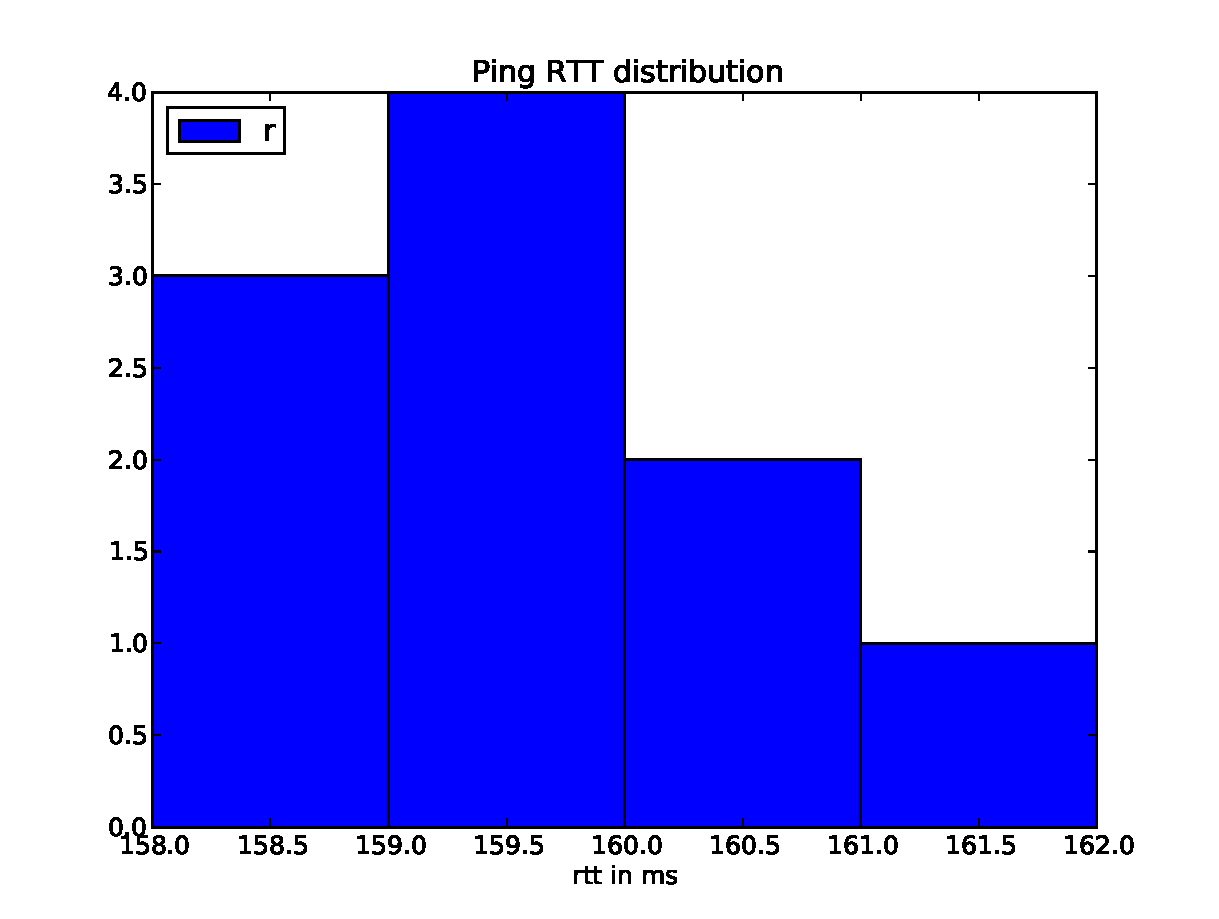
\includegraphics[height=4cm]{ping_distribution.pdf}   & 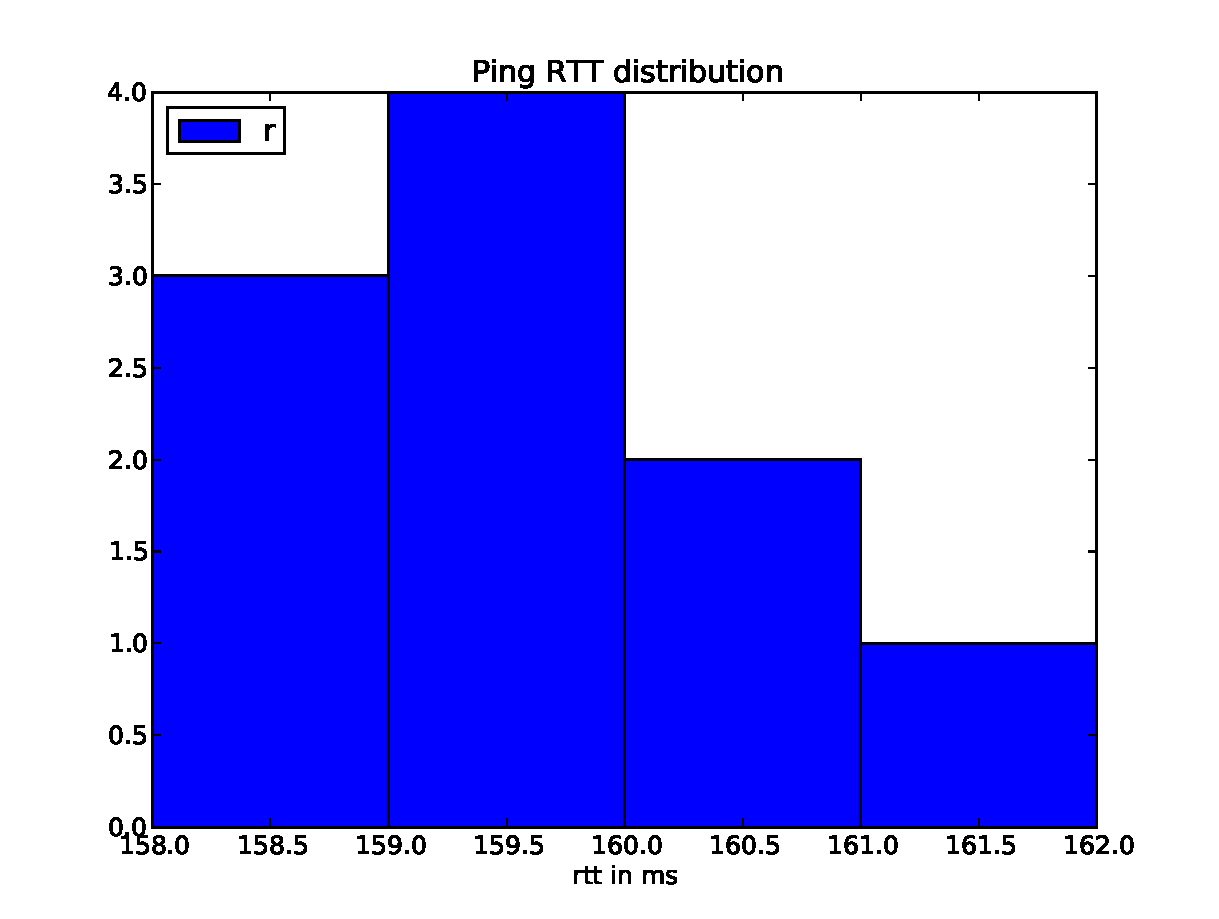
\includegraphics[height=4cm]{ping_distribution.pdf}  \\
\hline 
\end{tabular}
\end{table}
\end{pyframe}

\begin{pyframe}{Simple Column}
\begin{columns}
\column[t]{6cm}
\begin{pycode}
"""using set and dict
"""
distro = {x: rtt.count(x) 
  for x in set(rtt)}
# or using a
from collections import defaultdict
distro = defaultdict(int)
for x in rtt:
    distro[x] += 1
    

\end{pycode}
\column[t]{5cm}
-skip-\\
-skip-\\
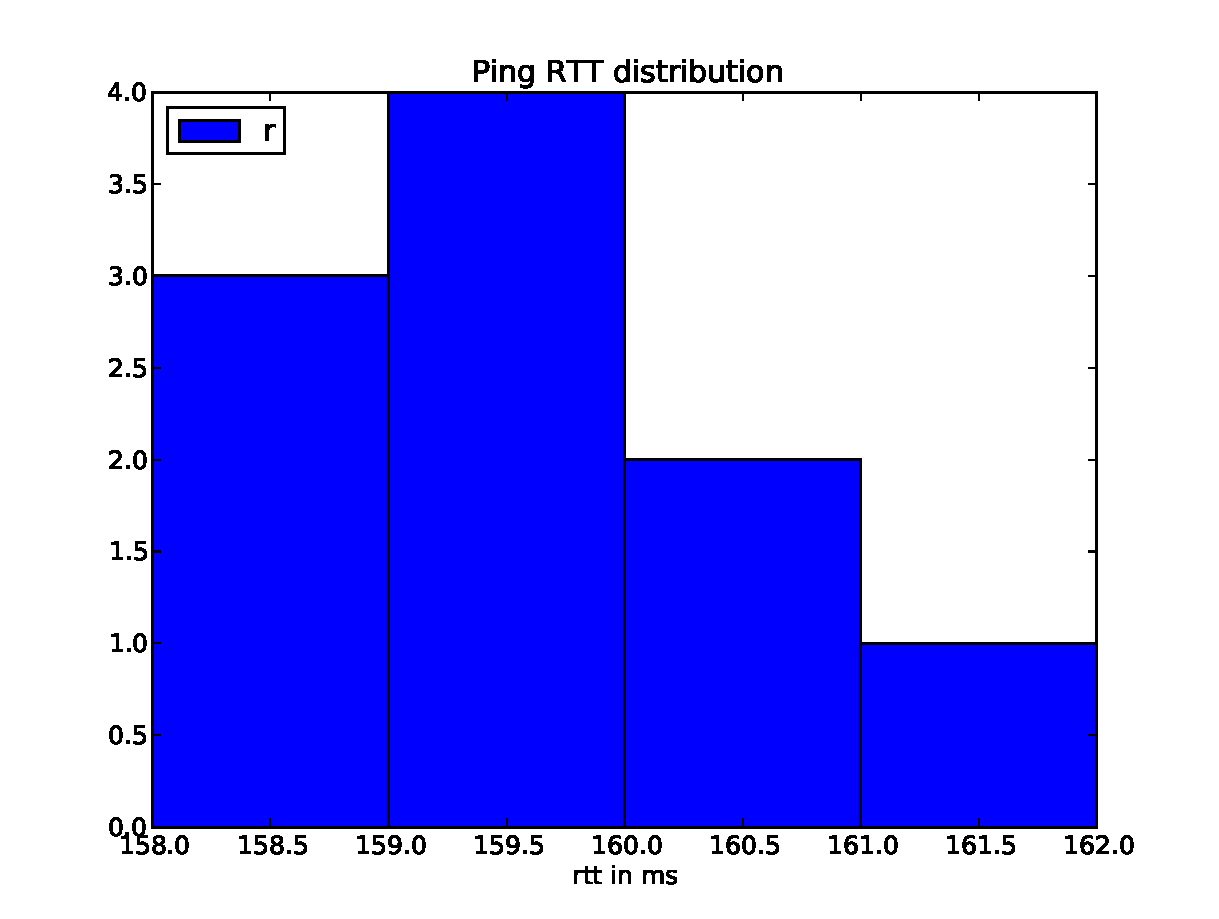
\includegraphics[height=4cm, width=4dm]{ping_distribution.pdf}  
\end{columns}
\end{pyframe}


\begin{pyframe}{2-columns and verbatim}
Two columns
\begin{columns}

\column[t]{5cm}
1
2
3
\begin{verbatim}
4
5
6
\end{verbatim}

\column[t]{5cm}
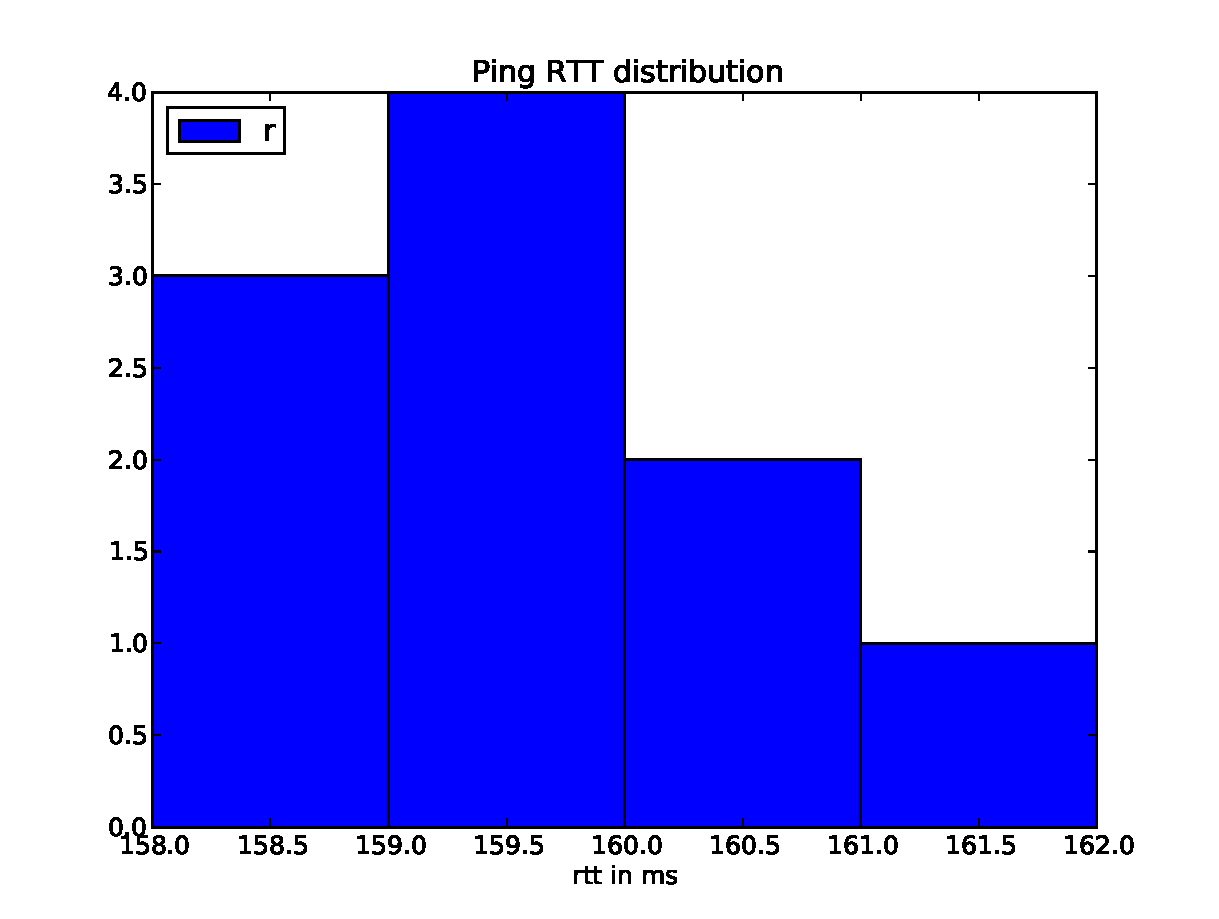
\includegraphics[height=4cm,width=5cm]{ping_distribution.pdf}  
\end{columns}

\end{pyframe}



\begin{pyframe}{Simple processing: distribution}
\begin{columns}
\column[t]{6cm}
\begin{pycode}
"""using set and dict """
distro = {x: rtt.count(x) 
  for x in set(rtt)}
# or using a
from collections import defaultdict
distro = defaultdict(int)
for x in rtt:
    distro[x] += 1
\end{pycode}
\column[t]{4cm}
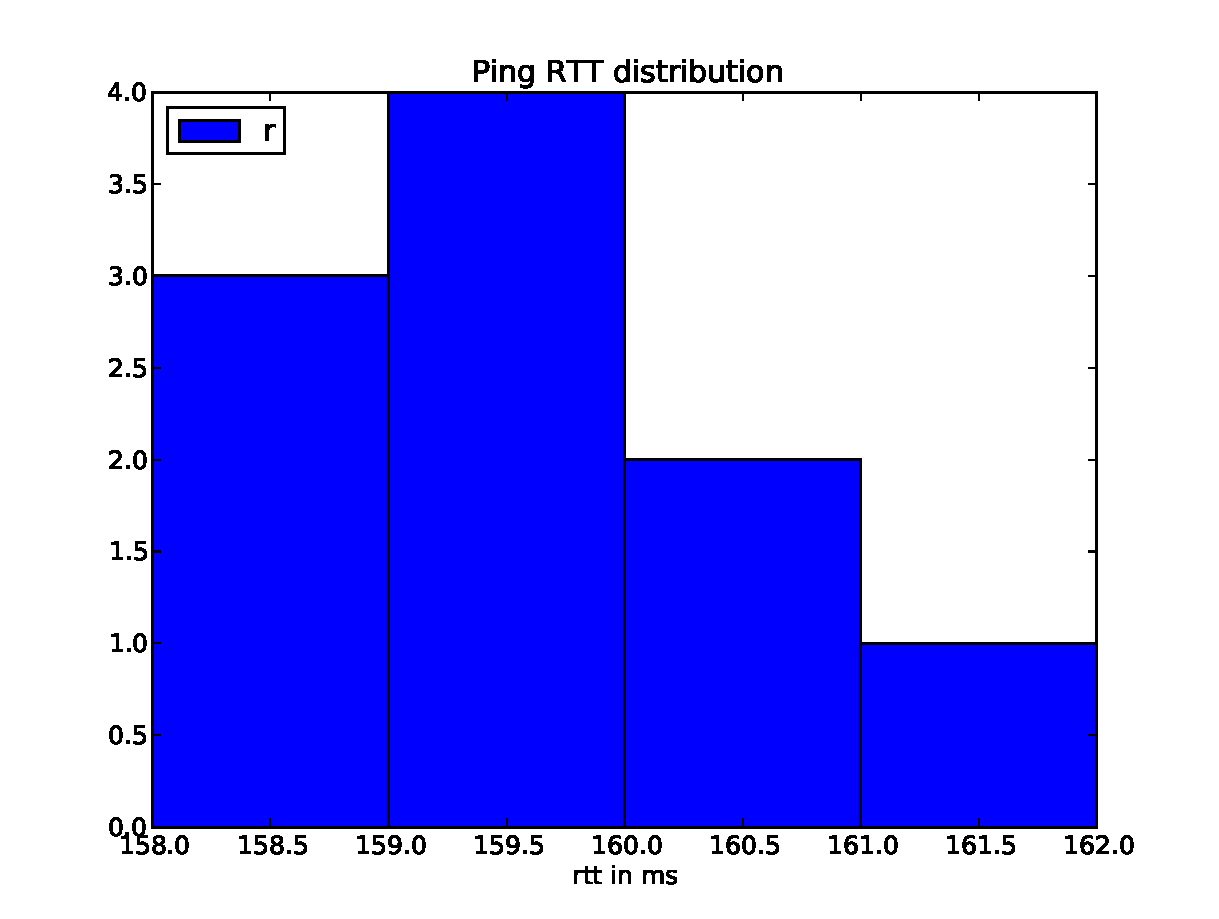
\includegraphics[width=4cm,height=4cm]{ping_distribution.pdf}  
\end{columns}
\end{pyframe}

\begin{pyframe}{Index}

fooo bar

\end{pyframe}



\section{Intro}
\frame{ \frametitle{Who? What? Why?}
\begin{itemize}

\item Use python to replace Grep Awk Sed Perl. Speed up your daily job.
\\

\item Roberto Polli - Solutions Architect @ par-tec.it. Loves writing in C,
Java and Python. Red Hat Certified Engineer and Virtualization
Administrator.
\\

\item Par-Tec – Proud sponsor of this talk ;) Contributes to various FLOSS and
provides expertise in IT Infrastructure \& Services and Business Intelligence
solutions + Vertical Applications for the financial market.

\end{itemize}
}


\begin{pyframe}{Requirements}
\begin{itemize}
\item python 2.7+, ipython

\item course code from github \\\\
\code{ \#git clone https://github.com/ioggstream/python-course}

\item test your environment (eg. psutil, numpy, scipy, matplotlib) \\\\
\code{ \#nosetests -vs test\_prerequisites.py }

\item first part: \pymodule{nose, psutil}
\item second part: \pymodule{scipy, numpy, matplotlib}
\item \pyoptional{optional/advanced content}
\end{itemize}
\end{pyframe}

\frame{ \frametitle{How}
\begin{itemize}
\item Get ready $before$ starting: code is \href{https://github.com/ioggstream/python-course/tree/master/python-for-sysadmin/README}{here on github}!

\item \emph{Type everything} but \code{\#comments} and \code{try/except}

\item \emph{Type fast} with tab-completion and copy-paste
% \emph{Type smart} with \code{\%edit testfile.py}!

\item Be curious: inspect and print returned variables

\item $Never^{*}$ close your iPython session: you'll lose your precious variables

\end{itemize}

* (ok, sometimes you can).
}

\begin{pyframe}{References}
\begin{itemize}
\item irc.freenode.net\# python - The Python Community :D
\item Python Cookbook 3rd ed. O'Reilly - David Beazley and Brian K. Jones
\item Programming Python 4th ed. O'Reilly - Mark Lutz
\item Dive into Python3 2nd ed. Apress - Mark Pilgrim
\item nose.readthedocs.org
\item github.com/ioggstream/python-course
\end{itemize}
\end{pyframe}


\begin{pyframe}{A Communication Issue}
- A message-forwarding infrastructure
- Episodic delays on some nodes
- Logs traces: message size, #peers, errors, retries
- Find the conditions related to the delays
\end{pyframe}


\begin{pyframe}{Gathering data}
The most time-consuming part of the analysis
- Parse log file with a strategy
- Collect log samples and tinker in ipython
- Write simple parsing library with tests
\end{pyframe}


\begin{pyframe}{Gathering data}
\begin{pycode}
# Use dict + zip to convert
data = [('timestamp', 'elapsed', 'error', 'retry', 'size', 'peers'),
(1379703191, 0.12, 2, 1, 123, 2313),
(1379703192, 12.43, 0, 1, 3223, 2303),
...
(1379 709000, 0.43, 0, 1, 3223, 2303)
]
# in
table = dict(zip(data[0],  zip(*data[1:]) ))
> { 'timestamp' : [ 1379703191, 1379703191, ..., 1379709000],
'elapsed': [0.12, 12.43, ..., 0.43],
... }

\end{pycode}
\end{pyframe}

\begin{pyframe}{Basic statistics}
Python provides basic statistics
\begin{pycode}
from scipy.stats import mean, std
print([k, max(v), min(v), mean(v), std(v) ] 
    for k,v in table.items() ])
\end{pycode}
\end{pyframe}


\begin{pyframe}{Distributions}
Data distribution shows event frequency. 
The plot shows a ping rtt distribution: the event is 
 expressed by range (eg. rtt in $[0,5)ms,[5,10)ms$)
\begin{pycode}
# The fastest way to get a distribution is
from matplotlib import pyplot as plt
frequency, values, _  = plt.hist(table['elapsed'])
zip(values, frequency)
\end{pycode}
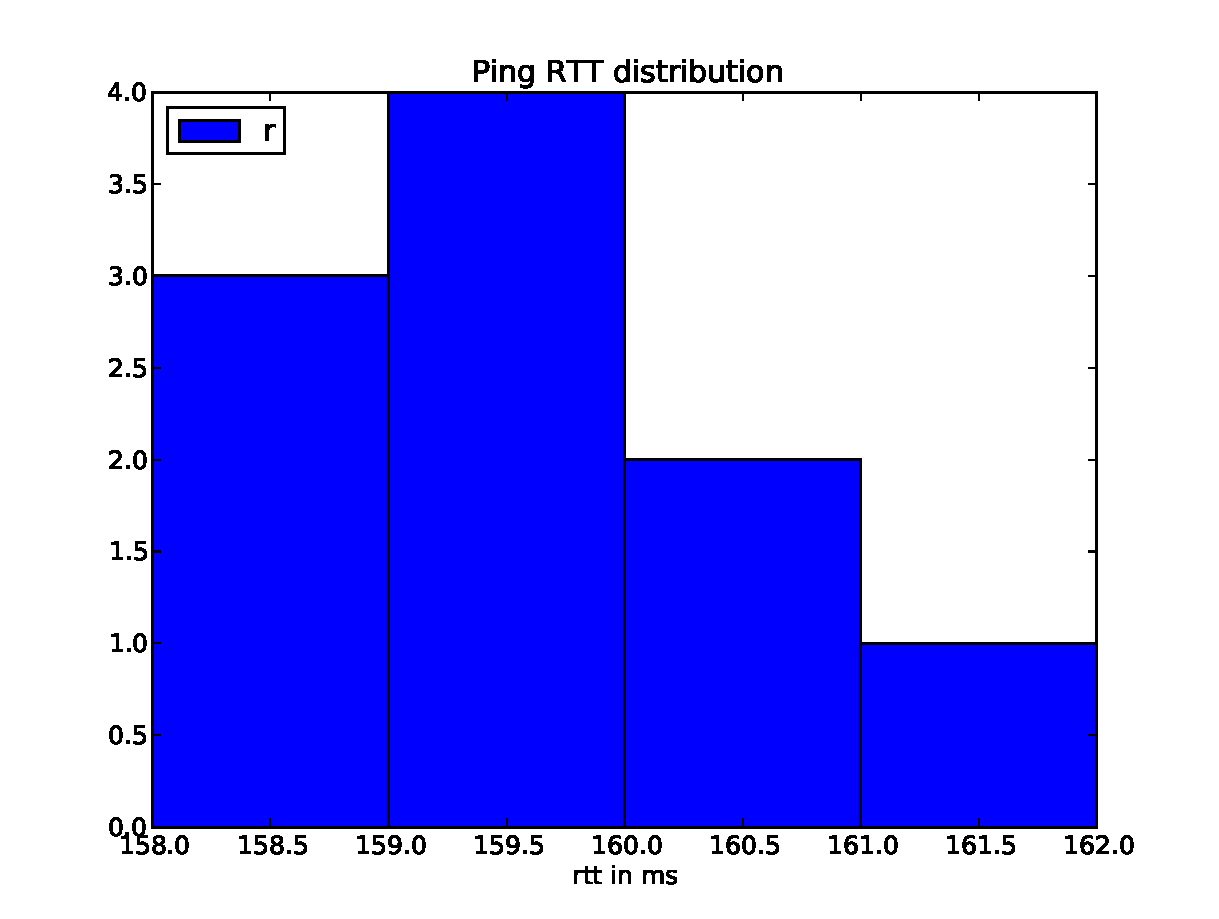
\includegraphics[width=5cm,height=5cm]{ping_distribution.pdf}
\end{pyframe}


\begin{pyframe}{Time and Size distribution}
Frequency can be calculate on time or size
Time distribution: mail sent in 4hours bucket
\begin{pycode}
from matplotlib import pyplot as plt
frequency, values, _  = plt.hist(table['elapsed'])
zip(values, frequency)
\end{pycode}
\includegraphics[width=5cm,height=5cm]{distribution.pdf}
\end{pyframe}





\end{document}
